\section{Odometry}
\label{sec:odometry}
Odometry is the process of measuring the travel of a vehicle. Using  a variety of sensor sources, the goal is to estiamte both the vehicle twist and its time integration, the later providing a full vehicle pose with respect to an initial frame called odometry. This initial frame is not attached to any physical entity, in contrast of map or vehicle frames, which are clearly related to a physical entity.

The word comes from the ancient greek, since there was a first invention of a device made by Archimides, which measured the path length run by a vehicle using a set of well calibrated gearboxes connected to the wheels\footnote{https://www.greecehighdefinition.com/blog/2019/4/14/ancient-greek-inventions-archimedes-odometer}. It was used to lay milestones to main routes. 

Odometry provides a smooth pose signal, an interesting feature for pose control, but suffers from a long-time drift, since its pose is usually computed as a time-integration of a noisy twist. Therefore, odometry is well suited for short-term feedback in trajectory control, but global correction is required for long-term route control.

\subsection{Twist integration in 2D}
Given a set of vehicle 2D twists at discrete time $t$, ~$\mathbf{u}^t=[v^t_x\ v^t_y\ w^t_z]^T$, expressed with respect to the vehicle frame at $t$, the time integration of these twists leads to a set of poses~$\mathbf{x^t}$, referenced to the initial vehicle frame.
\begin{figure}[bth!]
  \begin{center}
    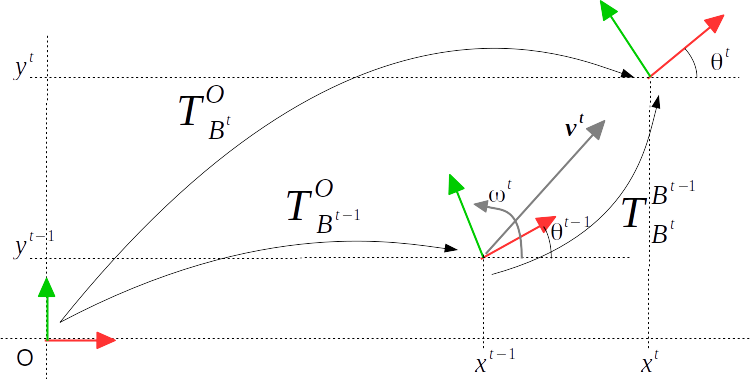
\includegraphics[width=1.0\columnwidth]{figures/odometry_integration_2d.png}
    \caption{Involved homogeneous transformations in the integration of a 2D twist. From pose at $t-1$, a twist composed of a linear velocity~$\mathbf{v}^t=[v^t_x\ v^t_y]$ and rotational velocity~$w^t_z$ is integrated to compute a pose at $t$.}
    \label{fig:odometry_integration_2d}
  \end{center}
\end{figure}

Figure~\ref{fig:odometry_integration_2d} shows the involved homogeneous transformations to compute the odometry poses. At a given discrete time $t-1$, the robot odometry pose is~$\mathbf{x^{t-1}}=[x^{t-1}\ y^{t-1}\ \theta^{t-1}]^T$, the transformation from the odometry frame up to the base (vehicle) frame is: 
\begin{equation}
 \mathbf{T}^O_{B^{t-1}} = 
 \left[
 \begin{array}{ccc}
  cos\theta^{t-1} & -sin\theta^{t-1} & x^{t-1} \\
  sin\theta^{t-1} &  cos\theta^{t-1} & y^{t-1} \\
  0 & 0 & 1
 \end{array}
 \right]
\end{equation}
At $t-1$ frame, the vehicle moves with a twist $\mathbf{u}^t=[v^t_x\ v^t_y\ w^t_z]^T$. Integrating this twist along a time increment~$\Delta\tau$, causes a pose increment expressed in vehicle frame at $t-1$, that can be represented by the following homogeneous transformation: 
\begin{equation}
 \mathbf{T}^{B^{t-1}}_{B^t} = 
 \left[
 \begin{array}{ccc}
  cos(w_z^t\Delta\tau) & -sin(w_z^t\Delta\tau) & v_x^t\Delta\tau\\
  sin(w_z^t\Delta\tau) &  cos(w_z^t\Delta\tau) & v_y^t\Delta\tau \\
  0 & 0 & 1
 \end{array}
 \right]
 \label{eq:odometry_increment}
\end{equation}
The product of the previous transformations leads to the new transformation that represents the new odometry pose at discrete time~$t$: 
\begin{equation}
\mathbf{T}^O_{B^t} = \mathbf{T}^O_{B^{t-1}} \cdot \mathbf{T}^{B^{t-1}}_{B^t}
\label{eq:odometry_transform_2D}
\end{equation}


\subsection{Uncertainty propagation in 2D}
Even if it comes from a filtering process, the twist is a noisy signal with a level of uncertainty. Therefore, the time integration explained in the previous subsection results in a pose with some degree of uncertainty too. To compute this uncertainty associated to the  odometry pose, given the twist unecrtainty, equation~\ref{eq:odometry_transform_2D} has to be linearized with respect to the twist components, prior to apply the uncertainty propagation seen at subsection~\ref{subsec:gaussian_uncertainty_propagation}: 
\begin{equation}
\mathbf{J}^{\mathbf{T}^{O}_{B^t} }_{v^t_x, v^t_y, \theta^t}= 
\mathbf{J}^{\mathbf{T}}_{\mathbf{u}} = 
 \left[
 \begin{array}{ccc}
  cos(w_z^t\Delta\tau) & -sin(w_z^t\Delta\tau) & v_x^t\Delta\tau\\
  sin(w_z^t\Delta\tau) &  cos(w_z^t\Delta\tau) & v_y^t\Delta\tau \\
  0 & 0 & 1
 \end{array}
 \right]
 \label{eq:odometry_jacobian}
\end{equation}

If the twist covariance matrix ~$\mathbf{C}^t_{\mathbf{u}}$, and the pose covariance matrix at previous iteration was~$\mathbf{C}^{t-1}_{\mathbf{x}}$, then the pose covariance at discrete time~$t$ is: 
\begin{equation}
 \mathbf{C}^t_{\mathbf{x}} = \mathbf{C}^{t-1}_{\mathbf{x}} +  
    \mathbf{J}^{\mathbf{T}}_{\mathbf{u}}
    \mathbf{C}^t_{\mathbf{u}}
    (\mathbf{J}^{\mathbf{T}}_{\mathbf{u}})^T
\end{equation}

From the above equation, it can be seen how the uncertainty associated to the odometry pose grows over time, leading to an unbounded dead reckoning pose estimation.
%\footnote{https://en.wikipedia.org/wiki/Dead_reckoning}

\subsection{Twist integration in 3D}
Given a set of vehicle 3D twists at discrete time $t$, ~$\mathbf{u}^t=[v^t_x\ v^t_y\ v^t_z\ w^t_x \ w^t_y \ w^t_z]^T$, expressed with respect to the vehicle frame at $t$, the time integration of these twists leads to a set of poses~$\mathbf{x^t}=[\mathbf{p}^t\ \mathbf{q}^t ]=[p^t_x\ p^t_y\ p^t_z\ q^t_r\ q^t_i\ q^t_j\ q^t_k]$, referenced to the initial vehicle frame. Conceptually, the integration process in 3D is the same as the process in 2D, but in terms of operations, 3D rotations allow to work in quaternion representation, so the integration equations are as follows: 
\begin{equation}
\mathbf{p}^t = \mathbf{p}^{t-1} + \mathbf{v}^t\Delta\tau
\end{equation}
for the position, and: 
\begin{equation}
\mathbf{q}^t = \mathbf{q}^{t-1}*\Delta\mathbf{q}^t
\end{equation}
for the orientation, where~$\Delta\mathbf{q}^t$ is the increment of quaternion due to rotational speed. Since~$\Delta\tau$ is usually a small time increment ($<10ms$), the rotation angle $\vert\mathbf{w}^t \vert \Delta\tau$ is usually also small, so  the increment of the quaternion can be approximated by: 
\begin{equation}
 \Delta\mathbf{q}^t \approx [1\ \frac{1}{2}w^t_x\Delta\tau\ \frac{1}{2}w^t_y\Delta\tau\ \frac{1}{2}w^t_z\Delta\tau ]^T
\end{equation}
and the orientation update can be also approximated by: 
\begin{equation}
\mathbf{q}^t = \mathbf{q}^{t-1}*\Delta\mathbf{q}^t
\approx 
\left[
 \begin{array}{cccc}
  1 & -\frac{1}{2}w^t_x\Delta\tau & -\frac{1}{2}w^t_x\Delta\tau & -\frac{1}{2}w^t_x\Delta\tau\\
  \frac{1}{2}w^t_x\Delta\tau & 1 & \frac{1}{2}w^t_x\Delta\tau & -\frac{1}{2}w^t_x\Delta\tau\\
  \frac{1}{2}w^t_x\Delta\tau & -\frac{1}{2}w^t_x\Delta\tau & 1 & \frac{1}{2}w^t_x\Delta\tau\\
  \frac{1}{2}w^t_x\Delta\tau & \frac{1}{2}w^t_x\Delta\tau & -\frac{1}{2}w^t_x\Delta\tau & 1\\
 \end{array}
 \right]
 \mathbf{q}^{t-1}
\end{equation}


\subsection{Inertial integration}
In case of using an Inertial Measurement Unit (IMU), odometry poses are computed by integrating accelerations and rotation rates read by accelerometers and gyroscopes respectively.


\subsection{Odometry sources}
There are several techniques that compute the list of poses referenced to the starting frame, called the odometry frame. They can be classified between three main approaches: (i) direct pose computation, (ii) twist time integration, (iii) inertial time integration. Table~\ref{tab:odom_sources} summarizes the main features of the most common approaches to solve the odometry problem, which is an active field in research. 
\begin{table}[hbt] \centering
\caption{Common techniques for odometry computation.}
\begin{tabular}
[c]{|c|c|c|c|c|c|c|c|}
\hline
\rowcolor{gray}    
Approach & Rate & Computational & Long-term & Short-term & Device & Typical \\
\rowcolor{gray}    
& & Complexity& drift & accuracy & mounting & application \\
\hline
Scan Matching & Low & High & Low & Medium & Delicate & Indoor \\
& & & & & & wheeled\\
\hline
Point Cloud & Low & Very High & Very Low & High & Delicate & Outdoor\\
registration & & & & & & wheeled\\
\hline
Visual & Medium & Very High & Very Low & High & Versatile & Space\\
Odometry & & & & & & Humanoids,\\
 & & & & & & Phones\\
\hline
Wheel & Medium & Low & Medium & Medium & Difficult & Wheeled\\
Encoders & & & & & & vehicles\\
\hline
Stereo & Low & Medium & Low & Medium & Rough & Automotive\\
Radar & & & & & & \\
\hline
IMU & High & Low & High & High & Versatile & Drones, \\
 & & & & & & Humanoids\\
\hline
\end{tabular}
\label{tab:odom_sources}
\end{table}

Please note that the above approaches show complementary features, therefore fusion of several approaches is highly recommended and leads to better results in both accuracy and robustness. 


